\documentclass[main.tex]{subfiles}
\begin{document}

\section{Results from Digital Setup and Performance Comparisson}
\subsection{Energy Calibrated QDC spectrum}
\begin{figure}[ht]
    \centering
        \includegraphics[width=\textwidth]{DigitalResults/Ecall.pdf}
        \caption{The 1.17 MeV edge of the $^60$ source and the 2.23 and 4.44 MeV Compton edges of the PuBe source have here been used to perform an energy calibration. Do to the event by event based baseline determination it is assumed that bin 0 corresponds to 0 $MeV_{ee}$}
    \label{fig:D_QDC}
\end{figure}



\subsection{Pulse shape discrimination}
\subsubsection{Charge comparisson method}
four parameters to tune: longgate and shortgate window and longgate and shortgate offset. Justify choice!
\begin{figure}[ht!]
    \centering
        \includegraphics[width=\textwidth]{DigitalResults/psd.pdf}
        \caption{The upper band consists mainly of neutrons. The 2.23 and 4.44 MeV gamma edges can clearly be seen in the gamma band below.}
        \label{fig:hex_a}
\end{figure}

\subsubsection{Convolutional neural network based discrimination}
To go in here: decision space, possibly saliency map.

\begin{figure}[ht!]
    \centering
        \includegraphics[width=\textwidth]{DigitalResults/CNN_E.pdf}
        \caption{}
    \label{fig:cnn_E} 
\end{figure}

\begin{figure}[ht!]
    \centering
        \includegraphics[width=\textwidth]{DigitalResults/tailTotal_vs_cnnPred.pdf}
        \caption{OLD data! On the x-axis we have the charge comparisson PSD parameter and on the y-axis we have the CNN prediction. The two classes seem to be better separated by the network.}
    \label{fig:tof_ps_d} 
\end{figure}

\subsection{Time of flight spectrum}
\begin{figure}[ht!]
    \centering
        \includegraphics[width=\textwidth]{DigitalResults/tof.pdf}
        \caption{The narrow peak is the gamma peak and the wider to the right is the fast neutron peak.}
    \label{fig:D_PSD_TOF} 
\end{figure}

\subsection{Pulse shape discrimination and ToF}
\begin{figure}[h!]
    \centering
        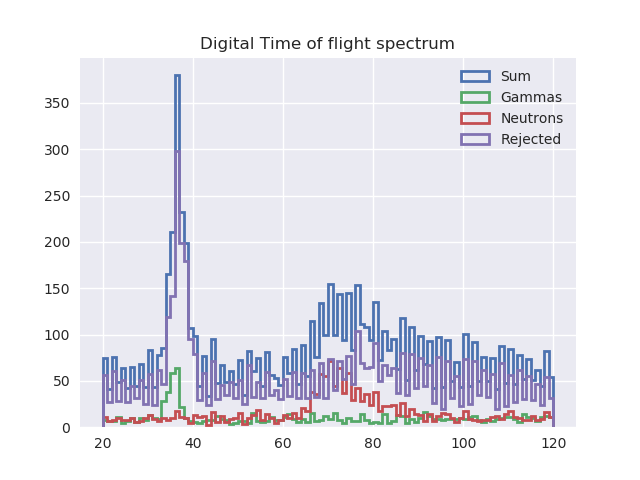
\includegraphics[width=0.8\textwidth]{DigitalResults/tof_psd.pdf}
        \caption{Plotting the tail/total ratio against the time of flight shows that what we are separating with this parameter is indeed neutrons and gammas. There is however some overlap.}
    \label{fig:tof_digi_cc} 
\end{figure}
\begin{figure}[h!]
    \centering
        \includegraphics[width=0.8\textwidth]{DigitalResults/ToF_vs_cnnPred.pdf}
        \caption{}
    \label{fig:tof_digi_cnn} 
\end{figure}


\begin{figure}
    \centering
    \begin{subfigure}[b]{\textwidth}
        \includegraphics[width=\textwidth]{DigitalResults/ToF_filt_CC.pdf}
        \caption{Time of flight spectrum filtered by a linear cut at tail/total=0.17.}
        \label{fig:tof_filt_cc}
    \end{subfigure}
	\begin{subfigure}[b]{\textwidth}
        \includegraphics[width=\textwidth]{DigitalResults/ToF_filt_CNN.pdf}
        \caption{Time of flight spectrum filtered by a linear cut at CNN prediction = 0.5.}
        \label{fig:tof_digi_filt_cnn}
    \end{subfigure}
    \caption{}
    \label{fig:animals}
\end{figure}




\end{document}